%%%%%%%%%%%%%%%%%%%%%%%%%%%%%%%%%%%%%%%%%%%%%%%%%%%%%%%%%%%%%%%%%%%%%%%%%%%%%%%%
%Objetivo: Introduzir os conceitos envolvidos na dissertação bem como do
%trabalho realizado. A ideia é que qualquer pessoa que leia a introdução
%consiga ter uma visão geral sobre a dissertação.
%Autor: Vagner Clementino<vagnercs@dcc.ufmg.br> e
%		Rodolfo Resende<rodolfo@dcc.ufmg.br>
%Criação: Dom Set 18 22:55:43 BRT 2016
%Modificação: qui mai 11 09:48:42 -03 2017
%Revisão: ter jun  6 19:27:28 -03 2017
%%%%%%%%%%%%%%%%%%%%%%%%%%%%%%%%%%%%%%%%%%%%%%%%%%%%%%%%%%%%%%%%%%%%%%%%%%%%%%%%
\chapter{Introdução}
\label{ch:intro}

% Dentro do ciclo de vida de um produto de software o processo de manutenção tem
% papel fundamental. Devido ao seu alto custo, que segundo alguns estudos varia
% entre 60\% a 90\% do preço final do software~\cite{kaur2015review}, as
% atividades relacionadas com manter e evoluir têm sua importância considerada
% tanto pela comunidade científica quanto pela indústria.Apesar da evolução das
% metodologias para se manter um software a estimativa é que nas últimas duas
% décadas o custo de manutenção tenha aumentado em
% 50\%~\cite{koskinen2010software}. Esta tendência pode ser observada na
% Figura~\ref{fig:software-maintence-costs} onde é possível verificar a evolução
% dos gastos com Manutenção de Software como fração do preço final do produto.

% Pelo menos desde a década de 1970~\cite{Zelkowitz:1979:PSE:578504} uma
% atenção %tem sido dada para os custos envolvidos com Manutenção de Software.
% Nas décadas %de 1980 e 1990 estudos propuseram modelos de mensuração do valor
% necessário para %manter o
% software~\cite{Herrin:1985:SMC:323287.323383,hirota1994approach}.

% \begin{figure}[htpb]
% \centering
% \includegraphics[width=0.6\linewidth]
% 				{./chapter-intro/img/software-maintence-costs.png}
% \caption{Evolução dos gastos com Manutenção de Software como razão do custo
%     total do projeto. Extraído de~\cite{engelbertink2010save}}
% \label{fig:software-maintence-costs}
% \end{figure}

Dentro do ciclo de vida de um produto de software o processo de Manutenção de
Software tem papel fundamental. Devido ao seu alto custo, que pode variar entre
60\% e 90\% do preço final do sistema~\cite{kaur2015review}, as atividades
relacionadas com manter e evoluir têm sua importância considerada tanto pela
comunidade científica quanto pela indústria. Uma vez que o software entra em
operação, anomalias são descobertas, mudanças ocorrem no ambiente de execução e
o atendimento à novos requisitos é solicitado. Estas atividades têm o apoio de
diversas ferramentas, dentre elas a que denominamos \texttt{Ferramentas de
    Gerenciamento de Requisições de Mudanças (FGRM)}. Esta dissertação apresenta
o estudo de FGRMs feito no correspondente projeto de mestrado e apresenta
contribuições sobre como melhorar este tipo de software.

A \textit{Manutenção}, dentre outros aspectos, corresponde ao processo de
modificar um componente ou sistema de software após a sua entrega com o objetivo
de \textit{corrigir falhas, melhorar o desempenho ou adaptá-lo devido à mudanças
    ambientais}~\cite{{159342}}. De maneira relacionada,
\textit{Manutenibilidade} é a propriedade de um sistema ou componente de
software em relação ao grau de \textit{facilidade} em que ele pode ser
corrigido, melhorado ou adaptado~\cite{{159342}}. As manutenções de software
podem ser divididas em \textit{Corretiva, Adaptativa, Perfectiva e
    Preventiva}~\cite{Lientz:1980:SMM:601062,159342}. A ISO 14764 discute as
quatro categorias e propõe que exista um elemento comum denominado
\textit{Requisição de Mudança (RM)} que representa as características
compartilhadas pelos demais tipos.

\begin{figure}[hbtp] \centering 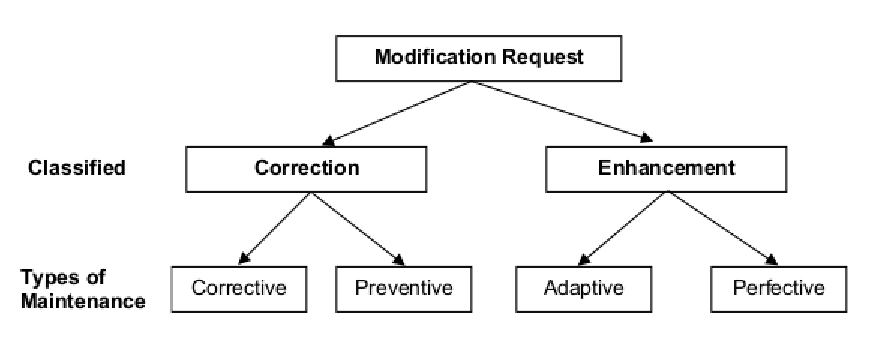
\includegraphics[width=.75\textwidth]
	{./chapter-intro/img/modification_request.eps} \caption{Tipos de manutenção
		segundo a norma ISO/IEC 14764. Extraído de~\cite{1703974}}
\label{fig:modification-request} \end{figure}

% Verificamos na literatura uma discussão sobre a diferença entre manutenção e
% evolução de software. Percebe-se ainda que pesquisadores e profissionais
% utilizam evolução como o substituto preferido para
% manutenção~\cite{Bennett:2000:SME:336512.336534}. Todavia, não está no escopo
% desta dissertação discutir e apresentar as diferenças entre os conceitos.
% Neste sentido, utilizamos os termos \textit{manter} e \textit{evoluir}
% software de forma intercambiáveis.

Por conta do volume das RMs, é importante a utilização de um software para
gerenciá-las. Esse controle é realizado pelas FGRMs que auxiliam o time de
manutenção na correção, de forma individual ou colaborativa, de falhas (bugs) ou
na implementação de melhorias. Estas ferramentas podem ser utilizadas por
gestores, analistas de qualidade e usuários do sistema mantido para atividades
como gerenciamento de projetos, comunicação, discussão e revisões de código. A
literatura sobre Manutenção de Software não define uma nomenclatura comum para
este tipo de software. Em alguns estudos são utilizados nomes como Sistema de
Controle de Defeito~-~Bug Tracking Systems, Sistema de Gerenciamento da
Requisição~-~Request Management System, sendo o mais comum o termo Sistemas de
Controle de Demandas (SCD)~-~Issue Tracking Systems. Todavia, de modo geral, o
termo se refere às ferramentas utilizadas no \textit{gerenciamento das
    Requisições de Mudança}. Nesta dissertação utilizamos o termo
\texttt{Ferramentas de Gerenciamento de Requisições de Mudança} (FGRM) ao
referimos a este tipo de software. A Tabela~\ref{tab:exemplo} apresenta alguns
exemplos de sistemas que podem ser classificados como FGRMs. Também são listados
serviços da Internet que oferecem funcionalidades existentes nas FGRMs na
modalidade de Software como Serviço~\cite{fox2013engineering}.

\begin{table}[htpb]
\centering
\resizebox{\textwidth}{!}{%
\begin{tabular}{@{}clll@{}}
\toprule
\multicolumn{2}{c}{Ferramentas}                   & \multicolumn{2}{c}{Serviços da Internet} \\ \midrule
Bugzilla & https://www.bugzilla.org/               & SourceForge  & https://sourceforge.net/  \\ \midrule
MantisBT & https://www.mantisbt.org/               & Lauchpad     & https://launchpad.net/    \\ \midrule
Trac     & https://trac.edgewall.org/              & Code Plex    & https://www.codeplex.com/ \\ \midrule
Redmine  & www.redmine.org/                        & Google Code  & https://code.google.com/  \\ \midrule
Jira     & https://www.atlassian.com/software/jira & GitHub       & https://github.com/       \\ \bottomrule
\end{tabular}%
}
\caption{Exemplos de ferramentas e serviços da Internet que podem ser
    classificados como FGRMs. Extraído de~\cite{cavalcanti2014challenges}}
\label{tab:exemplo}
\end{table}

\section{Motivação}
\label{sec:intro-motivacao}

Diante da maior presença de software em todos os setores da sociedade existe um
interesse por parte da comunidade científica e da industria no desenvolvimento
de processos, técnicas e \textit{ferramentas} que melhorem a relação
custo/benefício de manter um software. Dependendo do tamanho do projeto de
software é necessário a utilização de uma FGRM para gerenciar as suas
requisições de mudança. Além disso, as diferentes partes interessadas
(stakeholders) necessitam de um espaço único onde possam registrar as falhas
encontradas e as melhorias que necessitam~\cite{1407819}. Neste contexto,
verificamos que as FGRMs fazem parte de projetos de diferentes tipos e tamanhos,
em empresas públicas e privadas (por exemplo NASA e IBM) e de diversos projeto
de código aberto (por exemplo Mozilla, Eclipse, Apache); elas dão suporte à
softwares de diferentes plataformas: computadores de mesa (desktop), web ou
dispositivos móveis.

%Nesta linha, o trabalho de Yong \& Mookerjee~\cite{1423995} propõe um modelo que
%reduz os custos de manutenção e reposição durante a vida útil de um sistema de
%software. O resultado é que em algumas situações é \textit{melhor substituir um
    %sistema do que mantê-lo}. Este pro\-ble\-ma é agravado pelo fato de que, em
%alguns casos, são necessários 60\% dos desenvolvedores dedicados às tarefas de
%manutenção de sistemas~\cite{Zhang_2003}.

A literatura sobre FGRMs discute que a ferramenta desempenha um papel além do
gerenciamento dos pedidos de manutenção em software. Avaliando o controle de
demandas como um processo social, Bertram e
outros~\cite{Bertram:2010:CCB:1718918.1718972} realizaram um estudo qualitativo
sobre FGRMs que eram utilizadas por equipes de pequeno porte. Os resultados
demonstraram que a ferramenta era utilizada não apenas como um banco de dados de
rastreamento de falhas, mas atuava como um ponto central para a comunicação e
coordenação das diversas partes interessadas dentro e fora da equipe de
manutenção. Os clientes, gerentes de projeto, analistas de qualidade e
programadores contribuíam em conjunto para o compartilhamento do conhecimento do
projeto através da FGRM utilizada.

No trabalho de Breu e outros~\cite{Breu:2010:INB:1718918.1718973} o foco foi
analisar o papel das FGRMs no suporte à colaboração entre desenvolvedores e
usuários de um software. Com base nos resultados foi possível verificar que o
uso da ferramenta possibilitou que os usuários desempenhassem um papel além de
simplesmente reportar uma falha: a participação ativa e permanente foi
importante no progresso da solução das falhas que eles descreveram. Um outro
benefício das FGRMs é que as mudanças no software podem ser rapidamente
identificadas e reportadas para os desenvolvedores~\cite{anvik2005coping}. Além
disso, elas podem ajudar na estimativa do custo do software, na análise do
impacto de uma modificação, no planejamento do projeto, na rastreabilidade de
uma falha e na extração de conhecimento~\cite{cavalcanti2013bug}.

Conforme exposto, as FGRMs desempenham um papel fundamental no contexto do
desenvolvimento e manutenção de software. Entretanto, no escopo de sua
utilização diversos desafios se apresentam: duplicação de RMs, pedidos de
modificação abertos inadvertidamente, grande volume de RMs que devem ser
atribuídas aos desenvolvedores, RMs descritas de forma incompleta e
etc~\cite{cavalcanti2014challenges}. Diante destes problemas e desafios é
importante entender como estas ferramentas estão sendo utilizadas e o que está
sendo proposto na literatura sobre elas, de modo a avaliar e entender as
necessidades dos profissionais envolvidos com Manutenção de Software com o
objetivo de propor melhorias paras as funcionalidades oferecidas pelas FGRMs.

%No trabalho de Junio et al.~\cite{5741246} é proposto um processo denominado
%PASM (Process for Arranging Software Maintenance Requests) que propõe lidar com
%tarefas de manutenção como projetos de software. Para tanto, utilizou-se
%técnicas de análise de agrupamento (clustering) a fim de melhor compreender e
%comparar as demandas de manutenção. Os resultados demostraram que depois de
%adotar o PASM os desenvolvedores tem dedicado um tempo maior para análise e
%validação. De outra forma, relacionada um menor tempo foi dedicado às tarefas
%de execução e codificação.
%
%No estudo realizado por Bettenburg et al.~\cite{bettenburg2008makes} foi
%desenvolvida uma pesquisa (\textit{survey}) entre desenvolvedores e usuários
%dos projetos Apache\footnote{\url{http://www.apache.org/}},
%Eclipse\footnote{\url{https://www.eclipse.org}} e
%Mozilla\footnote{\url{https://www.mozilla.org}} a fim de verificar o que
%produziria uma boa FGRM\@. Os resultados demonstraram que do ponto de vista dos
%desenvolvedores eram consideradas úteis funcionalidades tais como reprodução do
%erro, rastros de pilhas (stack traces) e casos de testes. A partir deste
%resultado foi construído um protótipo capaz de conduzir os usuários na coleta e
%fornecimento de um maior número de informações úteis para a resolução do
%defeito reportado.
%
%
%Em Zimmermann et al.~\cite{5070993} é discutido a importância de que a
%informação descrita em uma Requisição de Mudança seja relevante e completa a
%fim de que o defeito reportado seja resolvido rapidamente. Contudo, na prática,
%a informação apenas chega ao desenvolvedor com a qualidade requerida após
%diversas interações com o usuário afetado. Com o objetivo de minimizar este
%problema os autores propõe um conjunto de diretrizes para a construção de um
%ferramenta capaz de reunir informações relevantes a partir do usuário e
%identificar arquivos que precisam ser corrigidos para resolver o defeito.
%

%No trabalho de Kononenko et al.~\cite{Kononenko:2014:DED:2591062.2591075} é
%apresentada uma ferramenta denominada \textit{DASH} cujo objetivo é agrupar as
%demandas que são relevantes para as atividades de um desenvolvedor.
%Naturalmente todas as demandas ditas relevantes deveriam estar sob a
%responsabilidade de um mesmo programador. O principal objetivo desta ferramenta
%é aumentar a Consciência Situacional (Situational Awareness) dos
%desenvolvedores. Segundo os autores, o principal ganho do uso da ferramenta é
%que os programadores podem gerenciar melhor o excesso de informação e ficar
%mais ciente da evolução das demais demandas do sistema.
%
%Na ferramenta proposta por Thung et al.~\cite{Thung:2014:DIT:2642937.2648627} o
%foco é na determinação de defeitos duplicados. A contribuição deste trabalho é
%a integração do estado da arte de técnicas não supervisionadas para detecção de
%falhas duplicadas conforme proposto por Runeson et
%al.~\cite{Runeson:2007:DDD:1248820.1248882}. A ferramenta utiliza o Modelo de
%Vetor Espacial (Vetor Space Model) como métrica de similaridade entre os
%defeitos e fornece aos desenvolvedores uma lista de possíveis duplicatas.

%A manutenção não necessariamente exige que o processo de software envolvido
%seja o tradicional. Percebe-se alguns exemplos de adoção das práticas ágeis
%para fins de manutenção e evolução do software~\cite{kajko2009model,
%Heeager2015, Devulapally2015,Naz2016}. Tal tendência não é surpreendente tendo
%em vista que os métodos ``ágeis'' enfatizam características úteis à eficiência
%da implementação de software, tais como desenvolvimento incremental e teste
%contínuo que agregam valor para a evolução e manutenção eficaz de um sistema
%\cite{thomas2006agile}. Dentro desta tendência verifica-se a necessidade de que
%as ferramentas envolvidas no suporte à manutenção de software se adéquem à este
%nova forma de manter software.
%

\section{Problema}
\label{sec:intro-problema}

O desenvolvimento e a manutenção de software envolvem diversos tipos de métodos,
técnicas e ferramentas. Em especial no processo de Manutenção, um importante
aspecto são as diversas RMs que devem ser gerenciadas, cujo controle é realizado
pelas FGRMs. Apesar da inegável importância dessa ferramenta, percebe-se um
aparente desacoplamento de suas funcionalidades com as necessidades das diversas
partes interessadas na manutenção e evolução de software. A utilização de
\textit{``demanda''} como conceito central para as FGRMs parece ser distante das
necessidades práticas dos projetos de software, especialmente no ponto de vista
dos desenvolvedores~\cite{Baysal:2013:SAP:2486788.2486957}.

%Contudo, em alguns casos, as ferramentas são
%meramente interfaces melhores para o banco de dados que armazena as
%RMs~\cite{zimmermann2009improving}.

Um exemplo deste desacoplamento pode ser visto no trabalho proposto por Baysal
\& Holme~\cite{baysal2012qualitative} no qual desenvolvedores que utilizam o
Bugzilla\footnote{\url{https://www.bugzilla.org}} relataram dificuldade em
manter uma compreensão do escopo que as RMs atribuídas para eles possuem.
Segundo eles seria importante que a ferramenta tivesse um suporte melhorado para
o conceito de Consciência Situacional~-~Situational Awareness. Em síntese, eles
gostariam de estar cientes da situação global do projeto bem como das atividades
que estavam sendo desempenhadas pelo demais desenvolvedores.

Existem outros prolemas que são potencializados pela ausência de certas
funcionalidades nas FGRMs. Uma amostra são as ferramentas que permitem a
inclusão de RMs com relatos de baixa qualidade. Nesta situação os usuários
terminam por serem questionados a inserir mais informação que algumas das vezes
não tem conhecimento. Por outro lado, verifica-se uma frustração por parte dos
desenvolvedores que não conseguem realizar o seu trabalho por conta da ausência
da informação que necessitam~\cite{just2008towards}.

Corroborando com a necessidade de evolução das FGRMs, o estudo realizado por
Zimmermann e outros~\cite{zimmermann2009improving} propõe quatro dimensões de
melhorias para este tipo de software. Estas dimensões representam
aperfeiçoamentos centrados em aspectos tais como \textit{ferramenta, informação,
    processo e usuário}. Eles são melhor discutidos no
Capítulo~\ref{ch:mapeamento-sistematico} em que foram utilizados na
classificação de estudos no Mapeamento Sistemático realizado.

% \begin{enumerate} [(i)]
% 	\item{Informação}
% 	\item{Processo}
% 	\item{Usuário}
% 	\item{Ferramenta}
% \end{enumerate}

Acreditamos que não é grande o número de trabalhos que avaliam de forma
sistemática as funcionalidades oferecidas pelas FGRMs, ao mesmo tempo que faça
relação com que vem sendo proposto na li\-te\-ra\-tu\-ra sobre o assunto.
Adicionalmente, os estudos sobre melhorias das FGRMs não discutem a adoção de
algumas das práticas propostas pelos agilistas na Manutenção de
Software~\cite{Soltan2016,Devulapally2015, Heeager2015}. É importante que as
FGRMs evoluíssem para se adaptar a esta forma de trabalho. Um outro fator que
corrobora sobre a necessidade de melhorias das FGRMs são as diversas extensões
(plugins) propostas na literatura
\cite{101186,Thung:2014:BIT:2635868.2661678,Kononenko:2014:DED:2591062.2591075}.

\section{Objetivos}
\label{sec:intro-objetivos}

Segundo o nosso entendimento existe um distanciamento entre as necessidades dos
profissionais envolvidos em Manutenção de Software e as funcionalidades
oferecidas pelas FGRMs\@. Por esta razão, este trabalho de dissertação investiga
e contribui no entendimento de como as FGRMs podem ser melhoradas ou estendidas
no contexto da transformação do processo de desenvolvimento e manutenção de
software de um modelo tradicional para outro que incorpora cada vez mais as
práticas propostas pelos agilistas. O intuito é analisar como as FGRMs estão
sendo modificadas com base na literatura da área em contraste com o ponto de
vista dos profissionais envolvidos com manutenção. Neste sentido, elaboramos um
estudo sobre as FGRMs com os seguintes objetivos:

\begin{enumerate}[(i)]
	\item entender os requisitos e funcionalidades oferecidas por este tipo de
        ferramenta;
	\item mapear as melhorias para as FGRMs que estão sendo propostas na
		literatura;
	\item avaliar sobre o ponto de vista dos profissionais a
		situação atual funcionalidades oferecidas pelas FGRMs\@;
	\item propor melhorias para as funcionalidades das FGRMs\@.
\end{enumerate}

%Vamos discutir os aspectos que são considerados mais importantes a partir da
%literatura da área, bem como do ponto de vista de profissionais envolvidos em
%manutenção de software. De forma particular, iremos estudar os mecanismos de
%personalização que algumas destas ferramentas permitem e tentaremos ainda criar
%exemplos de personalização para alguma possível extensão a ser identificada ao
%longo do trabalho.

\section{Visão Geral da Dissertação}
\label{sec:intro-visao-geral}

A fim de alcançarmos os objetivos descritos foi proposto um conjunto de
melhorias para as funcionalidades das FGRMs. As sugestões de aperfeiçoamento são
apresentadas no Capítulo~\ref{ch:sug_melhoria} e foram baseadas em um
\textit{(i)} mapeamento apresentado no Capítulo~\ref{ch:mapeamento-sistematico}
e em um \textit(ii) levantamento com profissionais descrito no
Capítulo~\ref{ch:pesquisa-profissionais}. O Capítulo~\ref{ch:sug_melhoria} além
de sugerir melhorias apresenta um levantamento da percepção destas recomendações
por parte de profissionais de desenvolvimento de software.

Mediante o mapeamento sistemático obtivemos e avaliamos uma parte das melhorias
para as funcionalidades das FGRMs que estavam sendo propostas na literatura. A
partir do estudo foi possível propor dois esquemas de classificação: por
dimensão de melhoria e suporte ao papel desempenhado na manutenção de software.
De maneira similar, através da caracterização das funcionalidade de algumas
FGRMs de código aberto ou disponíveis comercialmente, identificamos o estado da
prática deste tipo de ferramenta.

Com base nestes dois estudos conduzimos uma pesquisa com profissionais em que
pedimos que avaliassem os requisitos funcionais e não funcionais que poderiam
ser utilizados para aperfeiçoar as FGRMs. O questionário também quis saber a
opinião dos profissionais sobre a relevância das propostas de me\-lho\-ri\-as
existente na literatura em sua rotina de trabalho. Fundamentado nos estudos
descritos foi proposto um conjunto de melhorias. Percebemos que não tínhamos
tempo para implementar todas as nossas sugestões e escolhemos implementar apenas
uma delas conforme descrição do Capítulo~\ref{ch:implemtacao_extensao}.

\section{Metodologia de Pesquisa}
\label{sec:intro-metodologia}

% Alguns estudos descrevem quatro tipos de desenho em abordagens multi-método:
% embutido (embedded), exploratória, triangulada e
% explanatória~\cite{creswell2007designing}. Neste estudo, utilizamos uma
% abordagem de triangulação no qual consolidamos os resultados de diferentes
% métodos, considerando, contudo, que a mesma questão de pesquisa foi investigada
% em cada um deles. A utilização de um desenho triangular no trabalho melhora as
% conclusões e completude do estudo, trazendo maior credibilidade para os achados
% da pesquisa~\cite{hesse2010mixed}.

A metodologia de pesquisa utilizada neste estudo é baseada em uma abordagem
multi-método~\cite{hesse2010mixed}. Este tipo de desenho combina dois ou mais
métodos quantitativos ou qualitativos em um único estudo. Um estudo que faça uso
de um survey e um experimento é um exemplo deste tipo de
enfoque~\cite{hesse2010mixed}. As etapas do trabalho, que compõem a abordagem
multi-método estão listadas a seguir:

\begin{itemize}[(i)]
	\item Mapeamento Sistemático da Literatura~\cite{Petersen2008}
	\item Caracterização das funcionalidades das FGRMs
	\item Pesquisa (Survey) com os
		desenvolvedores~\cite{wohlin2012experimentation}
	\item Proposição e avaliação de um conjunto de melhorias para as FGRMs
    \item Implementação, como Prova de Conceito, de uma extensão para
        determinada FGRM
\end{itemize}

\section{Contribuições do Estudo}
\label{sec:intro-contribuicao}

Este estudo sistematizou uma parte da literatura sobre melhorias das
funcionalidades das FGRMs ao mesmo tempo que avaliou com base na opinião de
profissionais envolvidos com desenvolvido e manutenção de software a relevância
de tais alterações. Além disso, foi proposto um conjunto de recomendações que
podem contribuir com a melhoria das funcionalidades disponibilizadas por este
tipo de software. Uma das recomendações foi implementada demostrando a
aplicabilidade do que foi apresentado. Entendemos que uma FGRM que atenda as
necessidades dos desenvolvedores possa contribuir com o aperfeiçoamento das
atividades relacionadas com manutenção de software e diminuição de custos. Neste
sentido, entendemos que contribuímos no avanço dos estudos sobre melhorias das
FGRMs. Os resultados apresentados nesta dissertação podem ser utilizados para o
desenvolvimento de novas versões para este tipo de software ou serem aplicados
pela equipe de manutenção para otimizar a sua rotina de trabalho.

\section{Organização do Trabalho}
\label{sec:intro-organizacao-dissertacao}

Este trabalho de dissertação está organizado conforme descrito a seguir. No
Capítulo~\ref{ch:visao-geral-manutencao} apresentamos e discutimos os principais
conceitos utilizados nesta dissertação. Neste mesmo capítulo é descrito um
estudo em que coletamos as funcionalidades de um conjunto de FGRMs que foram
definidas como relevantes na visão de profissionais consultados mediante um
levantamento.

O Capítulo~\ref{ch:mapeamento-sistematico} descreve o mapeamento sistemático que
trata de trabalhos sobre melhorias nas funcionalidades das FGRMs. Os estudos
foram classificados em 04 dimensões de melhorias e pelo papel desempenhado na
Manutenção de Software que a melhoria visa dar suporte. No
Capítulo~\ref{ch:pesquisa-profissionais} reunimos a opinião de profissionais
envolvidos em Manutenção de Software sobre as funcionalidades oferecidas pelas
FGRMs. Estes profissionais exercem suas atividades em projetos de código aberto
e empresas do setor público e privado. Foi possível identificar que a maioria
dos participantes do levantamento estão satisfeitos com a ferramenta que
utiliza, contudo, eles se mostram interessados em novos tipos de funções para
este tipo de software.

Tomando como base a literatura sobre melhorias nas FGRMs e os resultados obtidos
nos estudos descritos em capítulos anteriores, apresentamos e discutimos um
conjunto de recomendações para as funcionalidades das FGRMs no
Capítulo~\ref{ch:sug_melhoria}. As sugestões propostas foram avaliadas por
profissionais que contribuem no desenvolvimento deste tipo de ferramenta. Em
geral, as recomendações tiveram boa aceitação com relação à sua necessidade e
facilidade de implementação. O Capítulo~\ref{ch:implemtacao_extensao} descreve a
implementação de uma das 8 sugestões propostas. O
Capítulo~\ref{ch:conclusao_trab_futuros} apresenta uma discussão final e também
apresenta algumas recomendações de trabalhos futuros.
